


\documentclass[11pt]{article}
\usepackage{geometry}                % See geometry.pdf to learn the layout options. There are lots.
\geometry{letterpaper}                   % ... or a4paper or a5paper or ... 
%\geometry{landscape}                % Activate for for rotated page geometry
%\usepackage[parfill]{parskip}    % Activate to begin paragraphs with an empty line rather than an indent
\usepackage{graphicx}
\usepackage{amssymb}
\usepackage{epstopdf}
\DeclareGraphicsRule{.tif}{png}{.png}{`convert #1 `dirname #1`/`basename #1 .tif`.png}

\title{Homework: Bayes Formula Exercise}
\author{Dan Beatty}
%\date{}                                           % Activate to display a given date or no date

\begin{document}
\maketitle
%\section{}
%\subsection{}

\section{Notes on problems}

How to use Bayes rule to generate loss and descriminate function.


\section{Problem 13}
\begin{quote}
	In many pattern classification problems one has the option either to assign the pattern to one of $c$ classes, or to reject it as being unrecognizable.  If the cost for rejects is not too high, rejection may be a desirable action.  Let 
\[
	\lambda ( \alpha _i | \omega_j) = 
\left\{
\begin{array}{ll}
0  &    i \equiv j  \\
\lambda_r  &    i \equiv c + 1  \\
\lambda_s  &   \textrm{ otherwise } 
\end{array}
\right.
\]
where 
\begin{itemize}
\item $i,j = 1,..., c$ 
\item $\lambda_r$ is the loss incurred for choosing the $(c+1)$th action, rejection
\item $\lambda_s$ is the loss incurred for making any substitution error.   
\end{itemize}
Show that the minimum risk is obtained if we decide $\omega_i$ if $P(\omega_i | \vec{x}) \ge P(\omega_j | \vec{x}) $  for all $j$ and if $P(\omega_i | \vec{x})  \ge 1 - \frac{\lambda_r}{\lambda_s} $, and reject otherwise.  What happens if $\lambda_r = 0 $?  What happens if $\lambda_r \ge \lambda_s$?  
\cite[68]{duda-hart-stork}
\end{quote}


\section{Problem 14}
\begin{quote}
	Consider the classification problem with rejection option
	\begin{enumerate}
		\item Use the result of Problem 13 to show that the following discriminant functions are optimal for such problems: 
		\begin{equation}\label{discriminantFunction}
			g_i(\vec{x}) = 
		\left\{
		\begin{array}{ll}
		p(\vec{x} | \omega_i) P(\omega_i)  &   i = 1, ..., c  \\
		\frac{\lambda_s - \lambda_r}{\lambda_s}  \sum _{j=1} ^ c p(\vec{x} | \omega_j) P(\omega_j) & i = c + 1 
		\end{array}
		\right.
		\end{equation}
		\item Plot these discriminant functions and the decision regions for the two-category one-dimensional case having two-category one-dimensional case having
		\begin{eqnarray}
			p(x | \omega_1) ~ N (1,1) \\
			p(x | \omega_2) ~ N(-1, 1) \\
			P(\omega_1) = P(\omega_2) = \frac{1}{2} \\
			\frac{\lambda _r}{\lambda_s} = \frac{1}{4}
		\end{eqnarray}
		\item Describe qualitatively what happens as $\frac{\lambda_r}{\lambda_s}$ is increased from 0 and 1. 
		\item Repeat for the case having:
		\begin{eqnarray}
			p(x | \omega_1)  ~ N(1,1) \\
			p(x | \omega_2) ~ N ( 0, \frac{1}{4}) \\ 
			P(\omega_1) = \frac{1}{3}, P(\omega_2) = \frac{2}{3} \\
			\frac{\lambda_r}{\lambda{s}} = \frac{1}{2}
		\end{eqnarray}
	\end{enumerate}
	
\cite[68]{duda-hart-stork}
\end{quote}
\subsection{Demo of optimization (aka part 1)}
In the case of acceptance under equation \ref{discriminantFunction}, $g_i(\vec{x})$ is monotonically increasing with $P(\omega_i | x)$, and $P(\omega_i |x)$ is monotonically increasing with the conditional risk.    

In the case of rejection, the value $\frac{\lambda_s - \lambda_r}{\lambda_s}$ the confidence factor, and greater than the greatest rejected $g_i(\vec{x})$.

\subsection{Plot these discriminant functions for the decision regions for the two-category one dimensional case.}

According to the two category method the plot of 
$g(x) = g_1(x) - g_2(x)$ in figure \ref{fig:exampleb2}  and plots of $g_1(x), g_2(x), g_r(x)$ in figure \ref{fig:exampleb1}
rejection is $g_1(x) < g_3(x)$ or $g_2(x) < g_3(x)$.  This occurs a rather steep point. 

\subsection{What happens to $g(x)$ as the confidence is altered}
The ratio $\frac{\lambda_r}{\lambda_s}$ allows more values of $x$ to be accepted the closer it gets to one.   The closer it is to zero, the more elements it rejects.  


\subsection{Plot for different values of $\sigma, \mu$}
See figures \ref{fig:example1}, \ref{fig:example2}, \ref{fig:example3}, \ref{fig:example4}

\begin{figure}[htbp] %  figure placement: here, top, bottom, or page
   \centering
   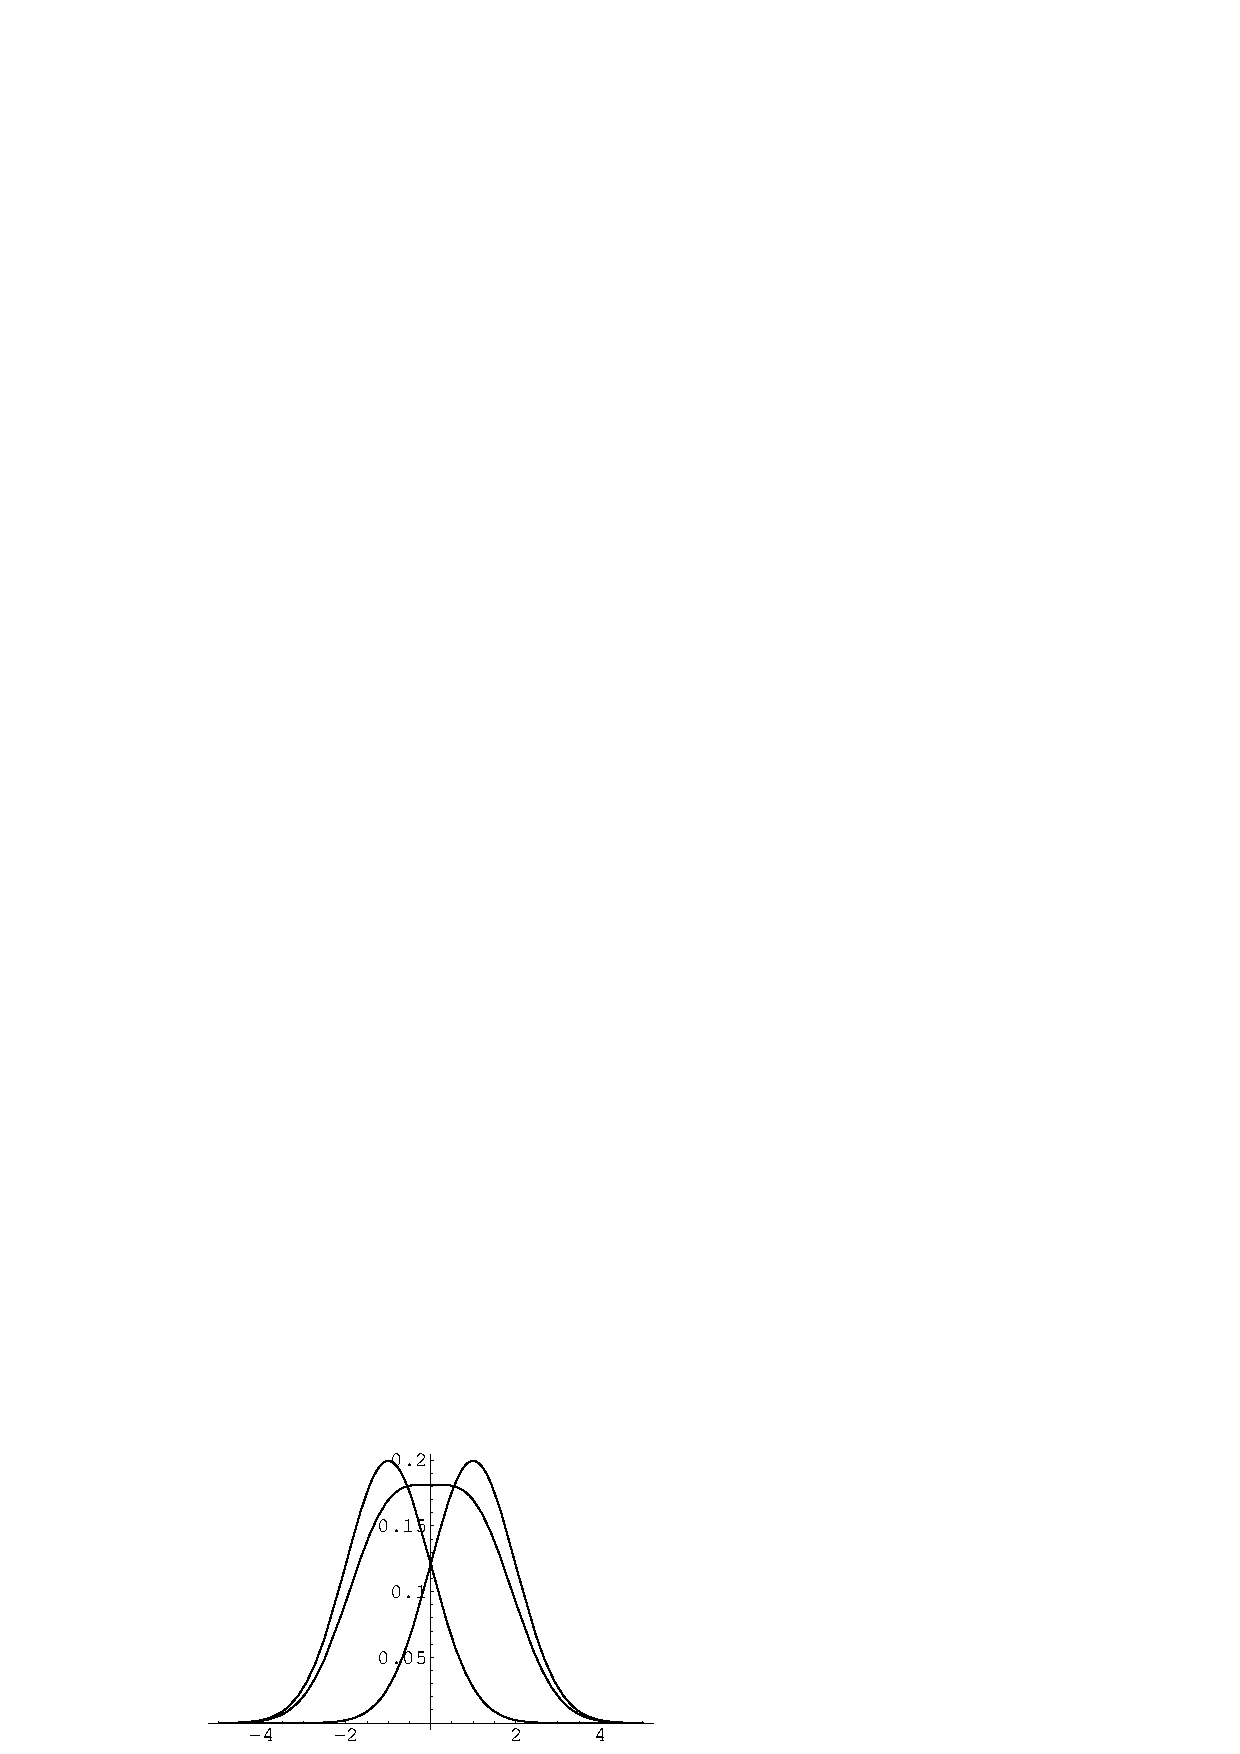
\includegraphics[width=2in]{partB_gr4.pdf} 
   \caption{Part B  $g_1(x), g_2(x), g_r(x)$}
   \label{fig:exampleb1}
\end{figure}


\begin{figure}[htbp] %  figure placement: here, top, bottom, or page
   \centering
   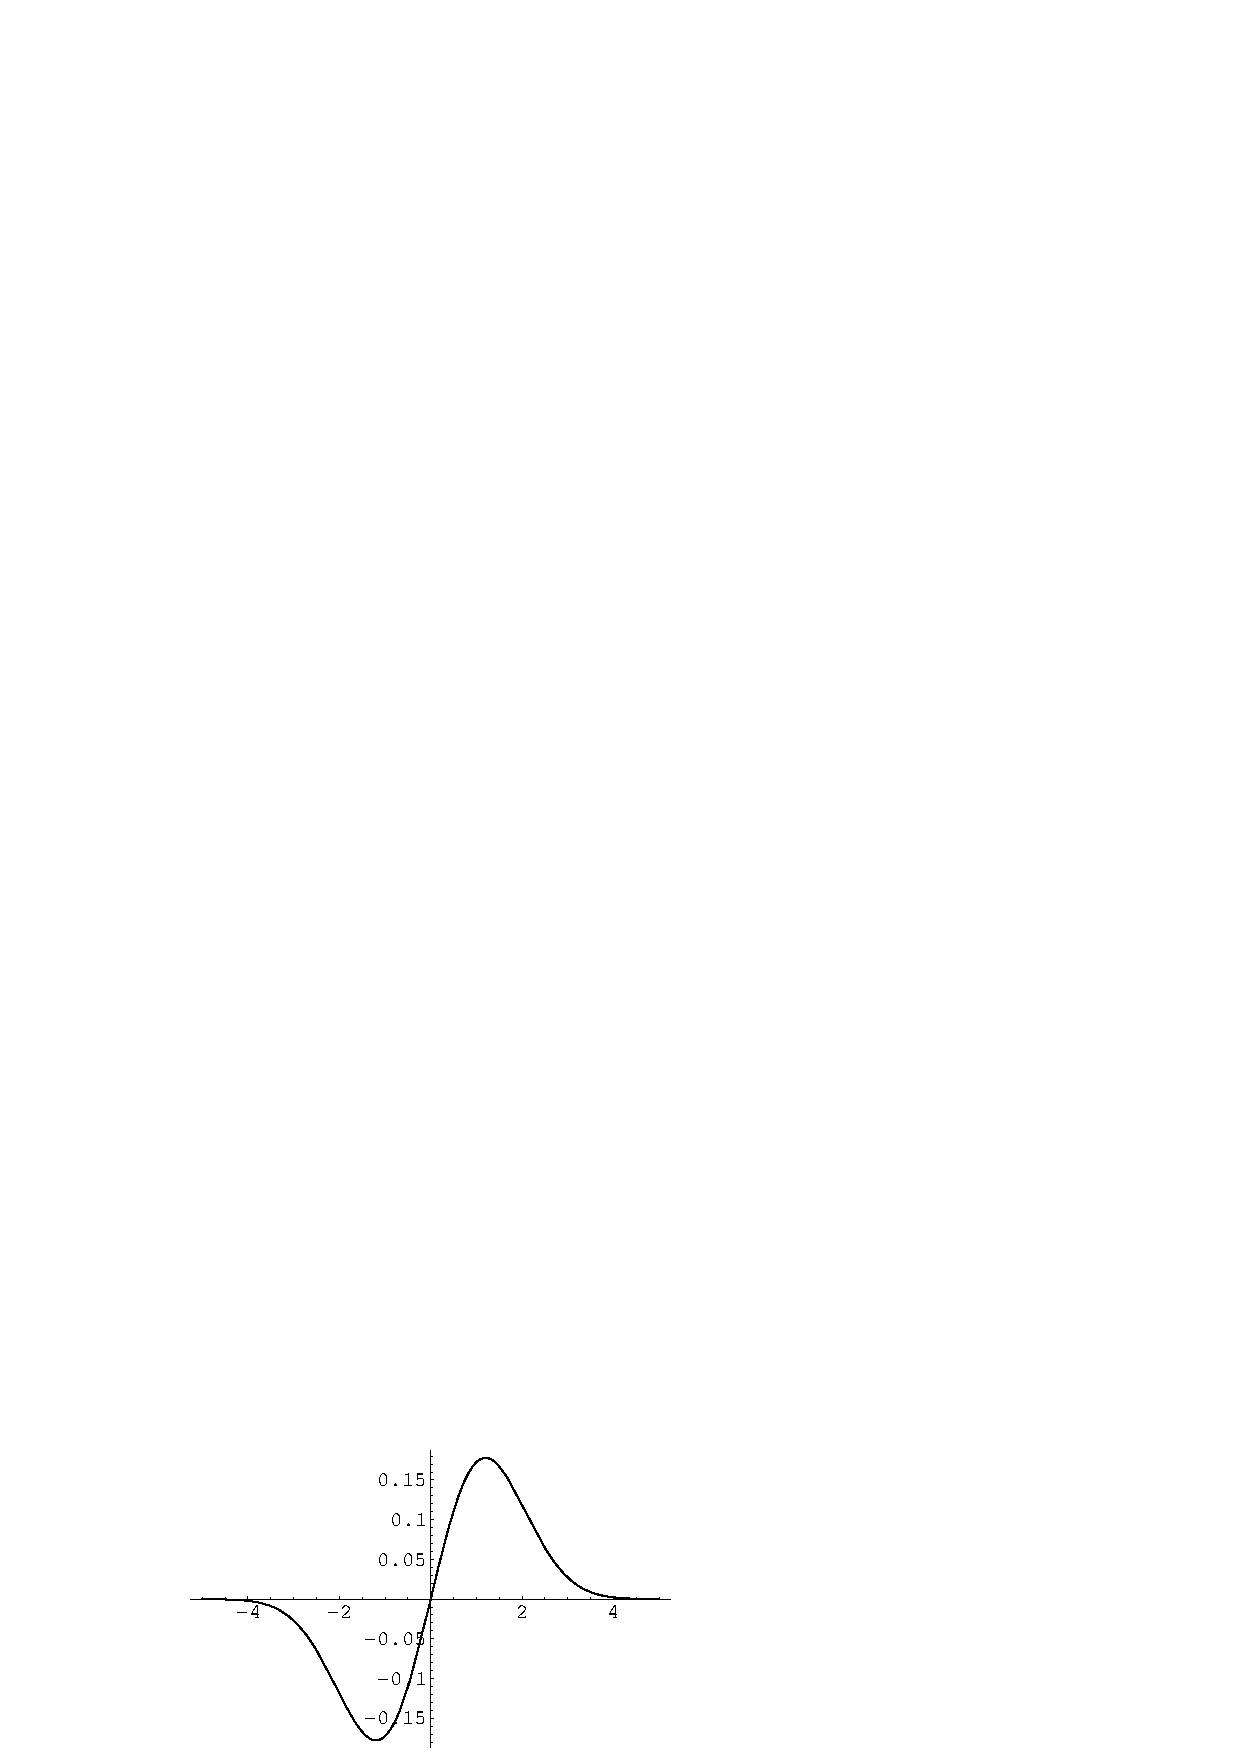
\includegraphics[width=2in]{partB_gr6.pdf} 
   \caption{Part B $g_1(x) - g_2(x)$}
   \label{fig:exampleb2}
\end{figure}




\begin{figure}[htbp] %  figure placement: here, top, bottom, or page
   \centering
   \includegraphics[width=2in]{partD_gr1.pdf} 
   \caption{Part D GR1}
   \label{fig:example1}
\end{figure}

\begin{figure}[htbp] %  figure placement: here, top, bottom, or page
   \centering
   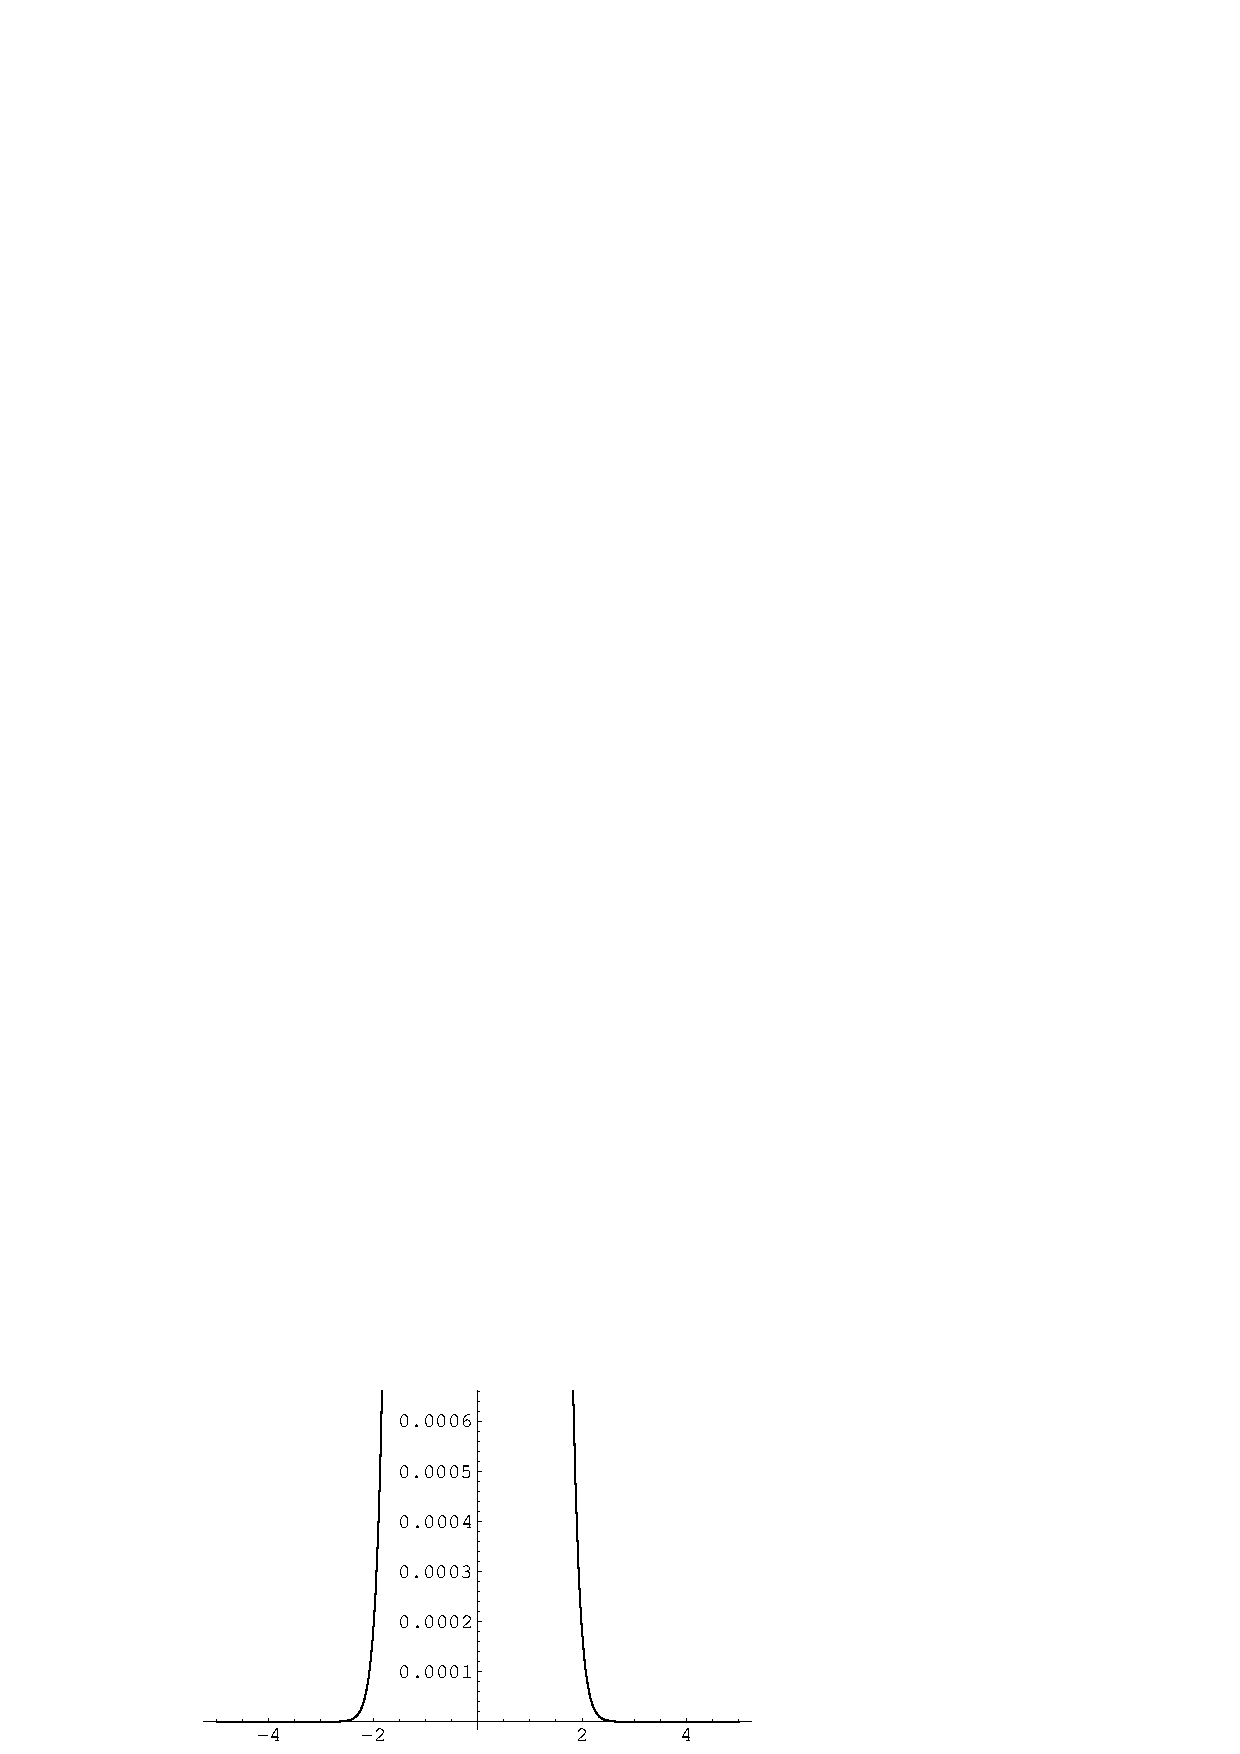
\includegraphics[width=2in]{partD_gr2.pdf} 
   \caption{Part D GR2}
   \label{fig:example2}
\end{figure}


\begin{figure}[htbp] %  figure placement: here, top, bottom, or page
   \centering
   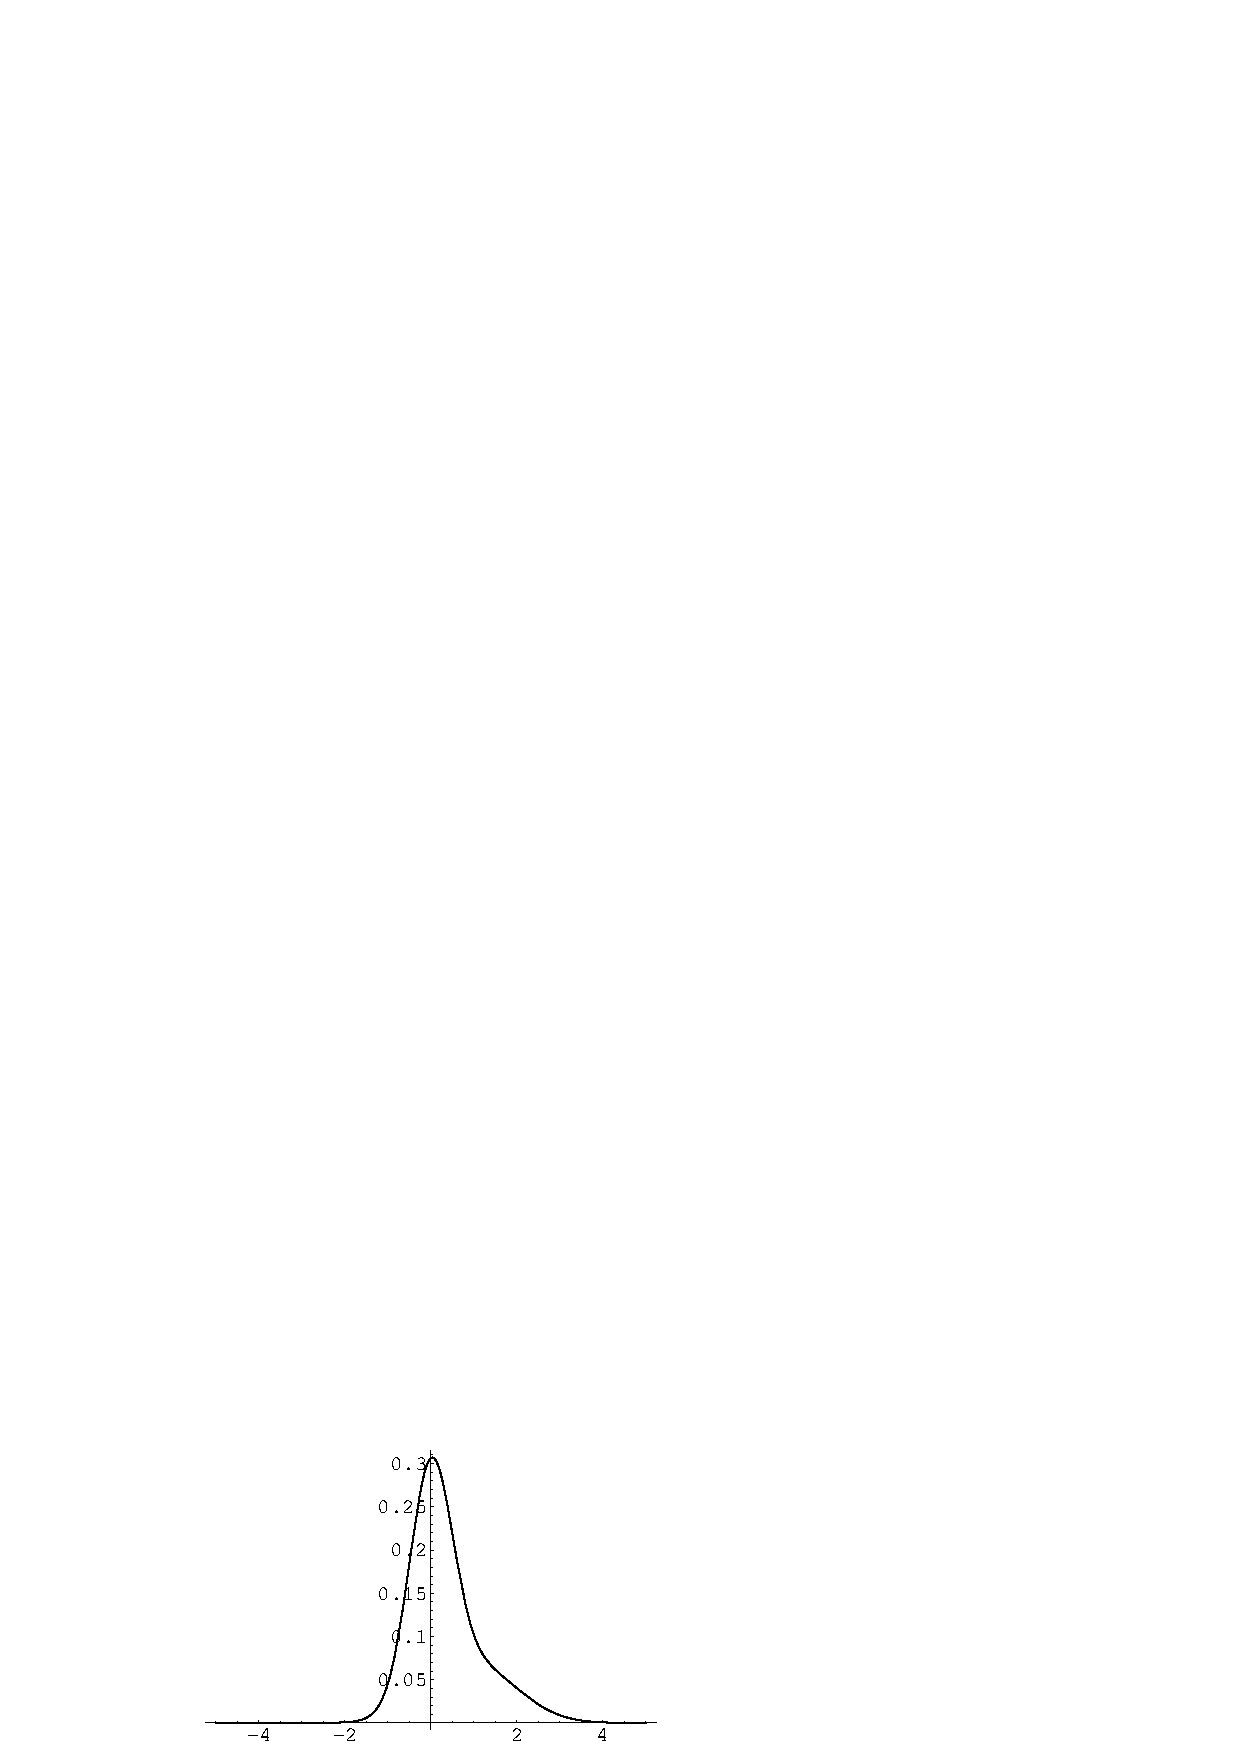
\includegraphics[width=2in]{partD_gr3.pdf} 
   \caption{Part D GR3}
   \label{fig:example3}
\end{figure}

\begin{figure}[htbp] %  figure placement: here, top, bottom, or page
   \centering
   \includegraphics[width=2in]{partD_gr4.pdf} 
   \caption{Part D GR4}
   \label{fig:example4}
\end{figure}


\bibliography{../patternNotes.bib}
\bibliographystyle{abbrv}
\end{document}  